\documentclass{article}

\usepackage[utf8]{inputenc}
\usepackage{hyperref}
\usepackage [english]{babel}
\usepackage [autostyle, english = american]{csquotes}
\MakeOuterQuote{"}
\hypersetup{
    colorlinks=true,
    linkcolor=blue,
    filecolor=magenta,      
    urlcolor=cyan,
}
\usepackage{xcolor}
\usepackage{listings}
\usepackage{inconsolata}
\definecolor{dkgreen}{rgb}{0,.6,0}
\definecolor{dkblue}{rgb}{0,0,.6}
\definecolor{dkyellow}{cmyk}{0,0,.8,.3}
\definecolor{pblue}{rgb}{0.13,0.13,1}
\definecolor{pgreen}{rgb}{0,0.5,0}
\definecolor{pred}{rgb}{0.9,0,0}
\definecolor{pgrey}{rgb}{0.46,0.45,0.48}
\lstdefinestyle{php}{
  language        = php,
  basicstyle      = \small\ttfamily,
  keywordstyle    = \color{dkblue},
  numbers=left,
  numberstyle=\tiny,
  numbersep=3pt,
  frame=tb,
  stringstyle     = \color{red},
  identifierstyle = \color{dkgreen},
  commentstyle    = \color{gray},
  emph            =[1]{php},
  backgroundcolor=\color{yellow!15},
  emphstyle       =[1]\color{black},
  emph            =[2]{if,and,or,else},
  emphstyle       =[2]\color{dkyellow}}
\lstset{showstringspaces=false}
\lstnewenvironment{php}
{\lstset{style=php}}
{}
\lstdefinestyle{java}{language=Java,
  showspaces=false,
  showtabs=false,
  breaklines=true,
  numbers=left,
  numberstyle=\tiny,
  numbersep=3pt,
  frame=tb,
  showstringspaces=false,
  breakatwhitespace=true,
  commentstyle=\color{pgreen},
  keywordstyle=\color{pblue},
  backgroundcolor=\color{yellow!15},
  stringstyle=\color{pred},
  basicstyle=\ttfamily,
  moredelim=[il][\textcolor{pgrey}]{$$},
  moredelim=[is][\textcolor{pgrey}]{\%\%}{\%\%}
}
\lstnewenvironment{java}
{\lstset{style=java}}
{}
\usepackage{graphics}
\usepackage{graphicx}
\usepackage{pdflscape}
\usepackage{afterpage}
\usepackage{capt-of}
% \usepackage{fontspec,fontawesome}
\graphicspath{ {images/} }

\title{FogBus Deep Learning Developer Tutorial - EdgeLens}

\author{Shreshth Tuli$^{1}$}
\date{June 2018}


\begin{document}
\maketitle

\section{Introduction}
This document includes the documentation of the code and insight on how different sections of the software can be tweaked or extended. All explanations and suggestions are based on the assumption that the reader has basic understanding of PHP and Python, and is well versed with programming concepts. \\
The document is divided into five major sections that deal with : 
\begin{itemize}
\item Master and Worker web interface (PHP)
\item Data Analyzer (Python)
\item Android Interface (MIT AI)
\item Functionalities of the Software
\item Further scope of development
\end{itemize}

\section{Web Interface}
All communication between the Fog nodes works using HTTP REST APIs, specifically GET and POST. 
\subsection{Master}
The Master performs the major tasks which include but are not limited to:
\begin{enumerate}
\item Take user login information and check with the Database
\item Maintain Database of registered users
\item Maintain configurations including Worker nodes' IP addresses
\item Take data for analysis
\item Distribute data with other parameters among worker nodes (or itself)
\end{enumerate}

\subsubsection{index.php}
The code snippet below of "index.php" shows the HTML form for taking the login information from the user and sending it using the POST method.
\begin{php}
<html>
<head><title>HealthKeeper - Login</title></head>
<body>

<!-- Title -->
<h1>HealthKeeper - Login Page</h1>

<!-- Login Form -->
<form id='login' action='index.php' method='post' 
accept-charset='UTF-8'>
<fieldset >
<legend>Login</legend>
<label for='username' >Username:</label>
<br>
<input type='text' name='username' id='username'  
maxlength="50" />
<br>
<label for='password' >Password:</label>
<br>
<input type='password' name='password' id='password' 
maxlength="50" />
<br><br>
<input type='submit' name='Submit' value='Submit' />
</fieldset>
</form>
\end{php}

The next snippet shows the database settings to connect with the MySQL database. As described in the "End User Tutorial", the settings include parameters like name of database (users), name of table (registrations). Using the $mysqli\_connect$ command, the web-server is able to connect to the required database. The database connection is indicated whether successful or not using 2 echo commands.\\ \\
Next the login information is checked using the SQL query to find entry with the entered credentials. If the number of rows is 1 then login is successful and the page navigates to "session.php" with GET tag of username. If login is not successful, then "Username or password incorrect" is displayed on the page.
\begin{php}
<?php
session_start();

// Database settings
$host = "localhost";
$user = "root";
$pass = "";
$db = "users";

// Connection to database
$dbConnected = mysqli_connect($host, $user, $pass, $db);
$dbSelected = mysqli_select_db($dbConnected, "users");
$dbSuccess = true;

// Show Database connection on screen
if($dbConnected){
	echo "MySQL Connection OK<br />";
	if($dbSelected){
		echo "DB Connection OK<br />";
	}
	else{
		echo "DB Connection FAIL<br />";
		$dbSuccess = false;
	}
}
else{
	echo "MySQL Connection FAIL<br />"; 
	$dbSuccess = false;
}

// Check login credentials
if(isset($_POST['username']) && isset($_POST['password']) 
&& $dbSuccess){
	$username = $_POST['username'];
	$password = $_POST['password'];
	$sql = "select * from registrations where 
    username='".$username."' AND
	password='".$password."' limit 1";
	$result = mysqli_query($dbConnected,$sql);
	if(mysqli_num_rows($result)==1){
		// Go to session page if login successful 
		echo "Login Successful!";
		header('Location: session.php/?username='.
        $_POST['username']);  
	}
	else{
		// Show incorrect credentials otherwise
		echo "Username or password incorrect!";
		exit();
	}
}
?>

</body>
</html>
\end{php}

\subsubsection{manager.php}
The "manager.php", handles all the worker IPs for the "session.php". It maintains the "config.txt", in which every line contains one IP address of a worker. "config.txt" also holds whether Master could be given the task of analysis or not. The following code snipper in the "manager.php", shows that if "Remove all Workers" is clicked, then "config.txt" is overwritten to a default state with no worker IP and Master enable to do the task.

\begin{php}
<?php

// Remove all worker nodes
if(isset($_POST['remove'])){
	file_put_contents("config.txt", "EnableMaster".PHP_EOL);
	echo "All Workers removed<br/>";
}
\end{php}
The next snippet shows how the config.txt is parsed. The method $fgets$, return a next line each time it is called. The while loop stores each line in the $\$content$ variable skipping the first line which contains the checkbox value. As per the "Enable Master" checkbox, the string "EnableMaster" or "DesableMaser" is added to $\$content$. 
\begin{php}
{
	// Read IPs from config.txt
	$file = fopen("config.txt", "r");
	$content = "";
	$line = fgets($file);
	while(($line = fgets($file)) !== false){
		$content=$content.$line;	
	}
	fclose($file);
	
	// Alter first line of config.txt as per 
    	// Enable master set or not
	if(isset($_POST['enable'])){
		file_put_contents("config.txt", 
        "EnableMaster".PHP_EOL.$content);
	}
	else{
		file_put_contents("config.txt", 
        "DisableMaster".PHP_EOL.$content);
	}
\end{php}
Whenever a new IP address is added, the POST tag \textit{\$\_POST[`ip']} is set and the IP is appended to the configuration file as shown in the snippet below.
\begin{php}
	// If new IP added, add to config.txt
	if(isset($_POST['ip']) && $_POST['ip']!=""){
	$file = fopen("config.txt", "a");
	$k = $_POST['ip']."\n";
	echo "Worker IP added : ".$_POST['ip']."<br/>";
	fwrite($file, $k);
	fclose($file);	
	
	}
\end{php}
The rest of the code displays the IPs set in the configuration file and lays down the form for adding new worker IP and the IP address of the local system (master).
\begin{php}
	// Display IPs already set
	echo "Set Worker IPs here <br/>";
	$file = fopen("config.txt", "r");
	$line = fgets($file);
	while(($line = fgets($file)) !== false){
		echo "Worker IP : ".$line."<br/>";	
	}
	fclose($file);
	echo "<br/>"."Add Worker IP<br/>";
	echo "
	<form id='ipinfo' method='post'>
	<input type='checkbox' name='enable' value='Yes' 
    	checked />
    	Enable Master as Worker <br/>
	<input type='text' name='ip' id='ip'  maxlength=\"500\" /> <br/>
	<input type='submit' name='add' value='Add Worker' /> <br/><br/>
	<input type='submit' name='remove' value='Remove all workers' />
	</form>";
	}
}
$localIP = getHostByName(getHostName());
echo "Master IP address : ".$localIP;
?>
<form id='login' action='home.php' method='post' accept-charset='UTF-8'>
<br><br>
<input type='submit' name='back' value='Go Back' />
</fieldset>
</form>

<?php
if(isset($_GET['username']))
{$user = $_GET['username'];}
else{$user = '';}
if(isset($_POST['back'])) {
	header('Location: ../home.php/?username='.$user); 
}

?>
</body>
</html>
\end{php}

\subsubsection{home.php}
The "home.php" is like a main menu page where the user can navigate to manager page or the session page. The code below shows how this is achieved.
\begin{php}
<html>
<head><title>HealthKeeper - Home</title></head>
<body>

<!-- Title -->
<h1>HealthKeeper - Home Page</h1>
<?php
session_start();
if(isset($_GET['username'])){
	$username = $_GET['username'];
	echo "<h2>Hello ".htmlspecialchars($username)."</h2> ";
}
else{
	echo "<h2>Hello</h2> ";
}
?>

<!-- Navigation Form -->
<form id='login' action='home.php' method='post' accept-charset='UTF-8'>
<input type='submit' name='manager' value='Go To Manager Page' />
&nbsp;&nbsp;&nbsp;&nbsp;
<input type='submit' name='session' value='Go To Session Page' />
<br><br>
<input type='submit' name='back' value='Go Back' />
</fieldset>
</form>

<?php
$user = $_GET['username'];

if(isset($_POST['manager'])){
	header("Location: ../manager.php/?username=".$user);	
}
elseif(isset($_POST['session'])) {
	header('Location: ../session.php/?username='.$user); 
}
elseif(isset($_POST['back'])) {
	header('Location: ../'); 
}
?>
</body>
</html>
\end{php}

\subsubsection{arbiter.php}
This performs the arbitration of the resources and gives the IP address of the worker node/ master node/ or cloud.

\begin{php}


<?php



session_start();
	
// Parse config.txt for IPs 
$file = fopen("config.txt", "r");
$line = fgets($file);
$choiceArray = explode(" ", $line);
$localIP = getHostByName(getHostName());
		
// Initialize choices
// true if work given to them, else false

$toMaster = true;	
if(preg_replace('/\s+/', '', $choiceArray[0]) == "DisableMaster"){
	$toMaster = false;	
}
$toAneka = true;	
if(preg_replace('/\s+/', '', $choiceArray[1]) == "DisableAneka"){
	$toAneka = false;	
}

$ips = array();
while(($line = fgets($file)) !== false){
  array_push($ips, $line);
}
	
// Initialize loads array to store loads of workers
$loads = array();
// For each IP, get load from load.php
foreach($ips as $ip){
	$ip = preg_replace('/\s+/', '', $ip);
	$dataFromExternalServer = @file_get_contents("http://".$ip."/EdgeLens/load.php");
	if($dataFromExternalServer != FALSE){
		$dataFromExternalServer =
		preg_replace('/\s+/', '', $dataFromExternalServer);	
		$my_var = 0.0 + $dataFromExternalServer;
		//echo "<br/>Woker load with IP ".$ip.": ".$my_var;
	} else{
		$my_var = 100;
	}
	array_push($loads, $my_var);	
	// If any load < 80% then toMaser and toAneka = false
  	if($my_var <= 0.8){
  		$toMaster = false;
  		$toAneka = false;
  	}
}
	
$result = "";

	
if($toMaster && $toAneka){
	$toAneka = false;
}

if(sizeof($loads) == 0){
	$toMaster = true;	
}	
	
if(!$toMaster && !$toAneka){
	// Work given to worker with least load
	$min = 100;
	$minindex = 0;
	foreach($loads as $load){
		if ($min > $load){
			$min = $load;			
		}		
	}
	foreach($loads as $load ){
		if($min == $load){
			break;			
		}		
		$minindex = $minindex+1;
	}
	$ipworker = $ips[$minindex];
	$ipworker = preg_replace('/\s+/', '', $ipworker);
	echo $ipworker;	
}
elseif($toAneka) {
	// Work done to Aneka
	$ipworker = "localhost";
	echo "cloud";
}
else{
	// Work done by master
	echo $localIP;
}

?>

\end{php}
Then, there is an HTML form for input of data from the user.

Next, if the "Analyze" button is clicked, then the content of "config.txt" is parsed to obtain list of worker IP addresses. The variable $\$toMaster$ stores if the task is to be given to the Master or not. It is initialized to false if first line in "config.txt" is "DisableMaster" and true otherwise.\\ \\
The next few lines form the code for the "Failover" and "Load Balancing" schemes of the software. The variable $\$ips$ is an array of the IP addresses and $\$loads$ is their corresponding loads. The PHP method $file\_get\_contents()$ allows us to get a string form of the webpage passed as the argument. The "@" operator with the $file\_get\_contents()$ is the error operator which lets it return $FALSE$ in case of errors. If any HTTP request for load returns FALSE then $\$my\_var$ is set to 100, and error message is displayed on the screen. Setting load to 100 has the effect that this node would never get the task and hence removed from load balancing IPs. The next time the worker IPs are accessed for load, this is checked again and if the particular worker node is available, it is taken into the load balancer. \\ \\
Using a for loop, the $\$loads$ array is populated by accessing the "load.php" of the corresponding IP address. If the load of any worker is < 80\%, then the variable $\$toMaster$ is set to false. In effect, when master is enabled as worker, this sets $\$toMaster$ to true only when all worker nodes have more that 80\% load.\\ \\
If the task is not given to the master, i.e. $\$toMaster$ is false, then the IP of the worker with minimum load gets the task. The task is sent using the GET method to the "worker.php" script of the worker with that IP address.  


\subsubsection{upload.php}
Uplaods the image for analysis

\begin{php}

<?php
   $data = file_get_contents('php://input');
   if (!(file_put_contents('input.jpg',$data) === FALSE)) echo "File xfer completed.";
   // file could be empty, though
   else echo "File xfer failed.";
?>
\end{php}

\subsubsection{exec.php}

This executes the YOLO code.

\begin{php}
<?php


if(isset($_GET["cloud"])){
	$file = fopen("cloud.txt", "r");
	$ip = fgets($file);

	move_uploaded_file("input.jpg", "input.jpg");
	$tmp = file_get_contents("http://".$ip."/EdgeLens/exec.php");
	
	echo $ip;
	exec("wget -O output.jpg http://".$ip."/EdgeLens/output.jpg");

}
else{
	echo exec("cp input.jpg ./Yolo/test/images/");

	while(true){
		if(file_exists("./Yolo/test/output/0_0.jpg")) break;
		else sleep(0.1);
	}

	echo exec("mv Yolo/test/output/0_0.jpg output.jpg");
}


echo "Done";

?>
\end{php}


\subsection{Worker}
The Worker node, displays CPU load, analyzes data and displays results. 

\subsubsection{load.php}
The "load.php" uses the PHP method : $sys\_getloadavg()$ to get the system CPU load and displays it.
\begin{php}
<?php
// Display CPU load
$load = sys_getloadavg();
echo $load[0];
?>
\end{php}

\subsubsection{manager.php}
The "manager.php" sets the Master IP address for data verification. It also displays the current set IP address of the Master which is saved in the configuration file (config.txt).
\begin{php}
<html>
<head><title>HealthKeeper - Manager</title>
</head>
<body>
<?php
if(isset($_POST['ip'])){
	// Set Master IP
	$file = fopen("config.txt", "w+");
	$k = "Master IP : ".$_POST['ip'];
	echo "Master IP Set to : ".$_POST['ip'].PHP_EOL;
	fwrite($file, $k);
	fclose($file);	
	
}
else{
	echo "Set Master IP here".PHP_EOL;
	$file = fopen("config.txt", "r");
	$k = fgets($file);
	echo $k.PHP_EOL;
	// Form to input Master IP
	echo "
	<form id='ip' method='post'>
	<input type='text' name='ip' id='ip'  maxlength=\"500\" />
	</form>";
	echo 	"<form id='Change IP' method='post'>
	<input type='submit' name='Change IP' value='Change IP' />
	</form>";
	fclose($file);

}
?>
</body>
</html>
\end{php}

\subsubsection{worker.php}
The "worker.php" script receives data to be analyzed using the GET method. It saves the data in "data.txt" and sets the first line to "Analysis Done = false". The Java based analysis application parses this data, saves results in "result.txt" and changes the first line of "data.txt" to "Analysis Done = true". This script once data has been written waits for the first line to change to "Analysis Done = true", and when so parses the result file. The result file's first line contains two parameters for analysis:
\begin{enumerate}
\item Number of times the oxygen level went below 88
\item Least oxygen level
\end{enumerate}
The current analysis scheme determines the disease severity on the basis of the following thresholds of the first parameter:
\begin{itemize}
\item < 5 : None
\item between 5 and 15 : Mild
\item between 15 and 30 : Moderate
\item > 30 : Highly severe
\end{itemize}

\begin{php}
<html>
<head><title>HealthKeeper - Worker</title></head>
<body>

<?php
if(isset($_GET['data'])){
	
	// Write Data to file
	$content = $_GET['data'];
	$file = fopen("data.txt", "w+");
	fwrite($file, "Analysis Done = false".PHP_EOL);
	fwrite($file,$content.PHP_EOL);
	fclose($file);

	// Wait for analysis done
	$file = fopen("data.txt", "r");
	$k = fgets($file);
	while(!preg_match("/Analysis Done = true/", $k)){
		fclose($file);
		$file = fopen("data.txt", "r");
		$k = fgets($file);
		usleep(500000);
	}
	fclose($file);	
	
	// Read results and display
	$file1 = fopen("result.txt", "r");
	$result = fgets($file1);
	$array = explode(",", $result);
	$count = (int)$array[0];
	$min = (int)$array[1];
	echo "For 1 hour of sleep data<br />";
	echo "AHI (Apnea-hypopnea index) = ".$count."<br />";
	echo "Minimum Oxygen Level reached : ".$min."<br />";
	$sev = "";
	if($count < 5){
		$sev = "None";
	}
	elseif($count < 15){
		$sev = "mild";
	}
	elseif($count < 30){
		$sev = "moderate";	
	}
	else{
		$sev = "Highly severe!";	
	}
	echo "Disease severity : ".$sev;			
}
?>
</body>
</html>
\end{php}

\newpage

\section{Data Analyzer}
The YOLO code is developed in Python and has been derived from \url{https://github.com/ayooshkathuria/pytorch-yolo-v3}. T
\newpage

\section{Android Interface}

The android app "EdgeLens.apk" allows the android device to act as an intermediary between the Camera sensor and the Master server. Rather than sending data manually through the GET HTML form, this app records and sends data automatically. The app has been developed on an open source platform : "MIT App Inventor" which can be seen at this \href{http://appinventor.mit.edu/explore/}{link}. The source file for "EdgeLens.apk" can be found \textit{FogBus-DDL/Android/EdgeLens.aia}. \\ \\


\subsection{Session Screen}
The Session screen is the main screen that handles all interaction with the master server. The blocks below show the variable initializations and screen initializations:
\begin{figure}[h]
\centering % Center table
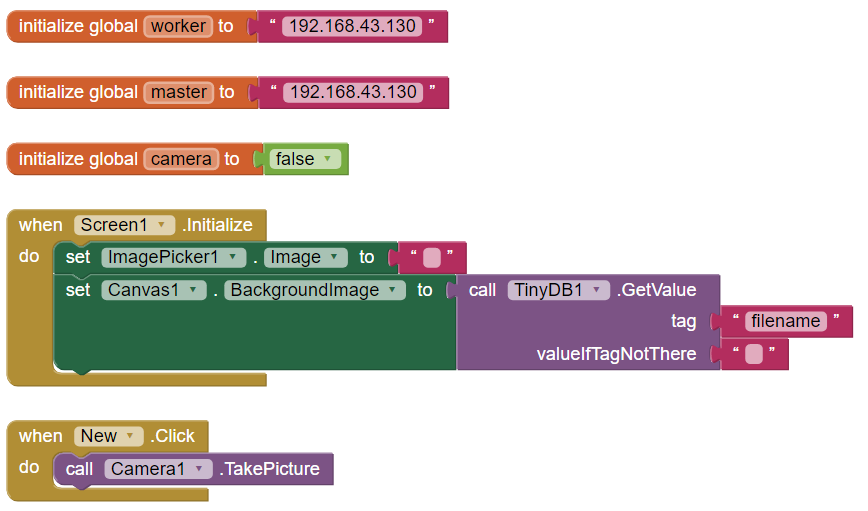
\includegraphics[width=\textwidth]{1.PNG}
\captionof{figure}{Session Screen block code}
\end{figure}

When a new image is clicked it is saved as "filename.jpg". When an existing image is picked, then it's path is saved. Canvas1 shows this image which is selected.
\begin{figure}[h]
\centering % Center table
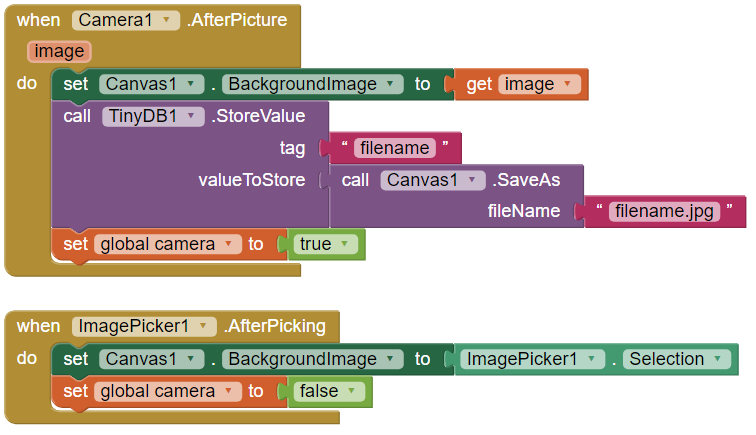
\includegraphics[width=\textwidth]{2.PNG}
\captionof{figure}{Session Screen block code}
\end{figure}


\begin{figure}[h]
\centering % Center table
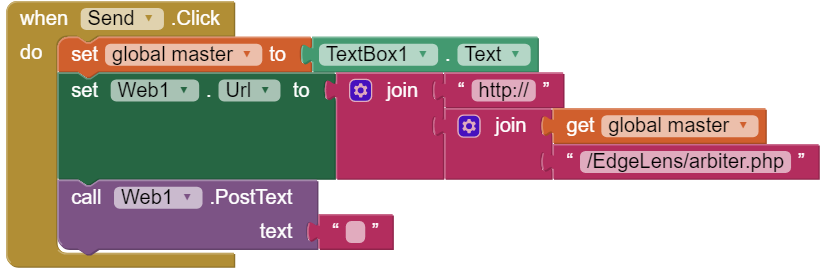
\includegraphics[width=\textwidth]{2-5.PNG}
\captionof{figure}{Session Screen block code}
\end{figure}

When the "Send" button is clicked then the Master's arbiter.php scripts is called in the Web veiwer to get the arbitration result. When the arbitration result is received then, the Canvas1 file is sent to the worker IP or Master IP without forwarding or Master IP with cloud forwarding indicated setting the \$GET['cloud'] to true.\\

\begin{figure}[H]
\centering % Center table
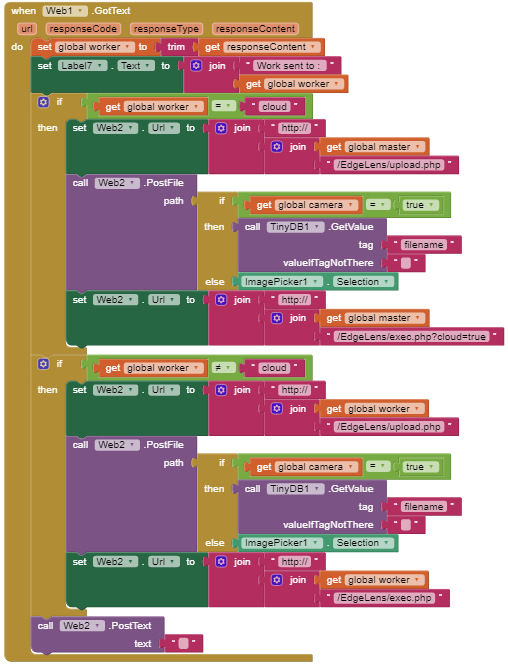
\includegraphics[width=\textwidth]{3.PNG}
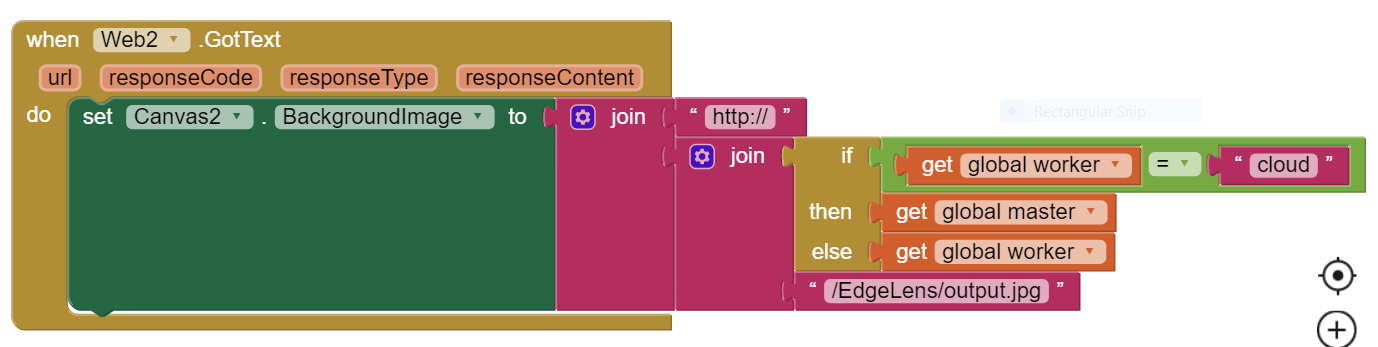
\includegraphics[width=\textwidth]{4.PNG}
\captionof{figure}{Session Screen block code}
\end{figure}

At last the results are retrieved and displayed in canvas2.

\newpage
\newpage


\section{Further Scope of developments}

This software form a base for setting up Fog Computing Environment which is not OS or architecture specific. Though the framework is complete by itself and fully functions to perform real-time, image object detection and segmentation, but has a large scope of improvement and further developments:
\begin{enumerate}
\item \textbf{Load Balancing Scheme} : As discussed earlier, the current load balancing scheme is naive and can be greatly improved. Currently, the load balancing scheme focuses on task distribution based on CPU load, whichever device has the least load, the task is given to it. There can be a cumulative ranking parameter which takes into account many other factors as per requirement. These factors can be and are not limited to : Network Bandwidth, Memory Load, etc. Different weights can given to these parameters are per the scenario.
\item \textbf{Data Integrity} : Health Analysis data is important for patients as their treatment and lives depend on it, thus it is important to save this data from fraudulent manipulation or sabotage from hackers. Thus, to maintain data integrity many techniques like Blockchain can be implemented to ensure that data is secure. 
\item \textbf{Data Privacy} : Some applications require data to be secure as well as kept private. The current system is prone to attacks and unwanted display of data to others. Privacy policies like encrypting the data can be used to ensure that the data can not be seen by others.
\item \textbf{Data Authenticity} : The current system allows any device to connect to master and share or view data. This can be used by hackers to forge DDoS or similar attacks. As Fog platforms also contains low range devices with limited threshold management, such attacks even at a low scale can destroy such devices. Thus a signature based validation technique can be used to ensure user and data authenticity. 
\end{enumerate}



\end{document}
